\documentclass[11pt]{report}
\usepackage[english]{babel}
\usepackage[utf8x]{inputenc}
\usepackage[T1]{fontenc}
\usepackage{lmodern}
\usepackage{amsthm}

\usepackage{color}
\usepackage{multirow}
%\usepackage{fourier-orns}
\usepackage{hyperref}
\newlength\myleftmargin
\setlength{\myleftmargin}{2cm}
\usepackage[margin=3.5cm, top=2.5cm, bottom=2cm,left=\myleftmargin,right=5.5cm,a4paper]{geometry}
\usepackage{graphicx}
\usepackage{caption}
\usepackage{array}
\usepackage{fancyvrb}
\usepackage{xparse}

\setlength{\parskip}{2mm}
\setlength{\parindent}{0pt}

\usepackage{enumitem}
\setlist[itemize]{noitemsep, topsep=0pt}

\newcounter{questionum}
\setcounter{questionum}{0}

% \renewenvironment{verbatim}{\tiny\color{gray}\VerbatimEnvironment\begin{Verbatim}}{\end{Verbatim}}
% \renewenvironment{verbatim}{\tiny\color{gray}\VerbatimEnvironment\begin{Verbatim}[lastline=1]}{\end{Verbatim}}

\newcommand\com[1]{\textsf{#1}}

\newcommand\question[1]{\refstepcounter{questionum}\par\noindent\textbf{\thequestionum}.~#1}
\setlength{\marginparsep}{1em}
\setlength{\marginparwidth}{4cm}

\newcommand\reponse[1]{\textcolor{white}{#1}}
\newcommand\fl{\,\ensuremath{\longrightarrow}\,}

\let\oldmarginpar\marginpar
\renewcommand\marginpar[1]{\oldmarginpar{\footnotesize\itshape #1}}

\usepackage{titling}

\usepackage{tikz}

\newcommand\new{%
  \tikz[overlay, remember picture]{\coordinate[anchor=base] (line) at (0,0);
    %
    \coordinate (margin start) at ([xshift=\myleftmargin]line -| current page.west);
    \node[anchor=base east, font=\bf] at (margin start) {New!};}}

\makeatletter
\renewcommand\maketitle{\begin{minipage}[c]{.7\textwidth}%
{\LARGE\sf \@title}
\\[1ex] \today
\end{minipage}
\hfill
\begin{minipage}[c]{.2\textwidth}
%\includegraphics[width=\textwidth]{grid-0}
\end{minipage}
}
\makeatother


\title{Mastering the Vidjil web application
}


\widowpenalty10000
\clubpenalty10000

\begin{document}

\begin{verbatim}
# coding: utf-8
load 'vidjil_browser.rb'
load 'browser_test.rb'

#browser test suite
class TestList < BrowserTest

  def setup
    super
    if not defined? $b
      set_browser("/browser/test/data/demo_lil_l3_tutorial.vidjil")
      if $b.div(id: 'tip-container').present?
        $b.div(:id => 'tip-container').div(:class => 'tip_1').element(:class => 'icon-cancel').click
      end
    end
  end

  # position of clones
  # clone 0, top clone of last sample (relapse)
  # clone 1, top clone of first sample
  # clone 4, second clone of first sample
  # clone 7, 11, 13; clone 3, 4 and 5 of first sample

  def after_tests
  end
\end{verbatim}


\maketitle

\textit{The goal of this practical session is to learn
common ways to visualize, filter, analyse and cluster clones
on the Vidjil web application.
%
These clones may have been computed by the Vidjil algorithm
or by any other algorithm.}

\bigskip


\centerline{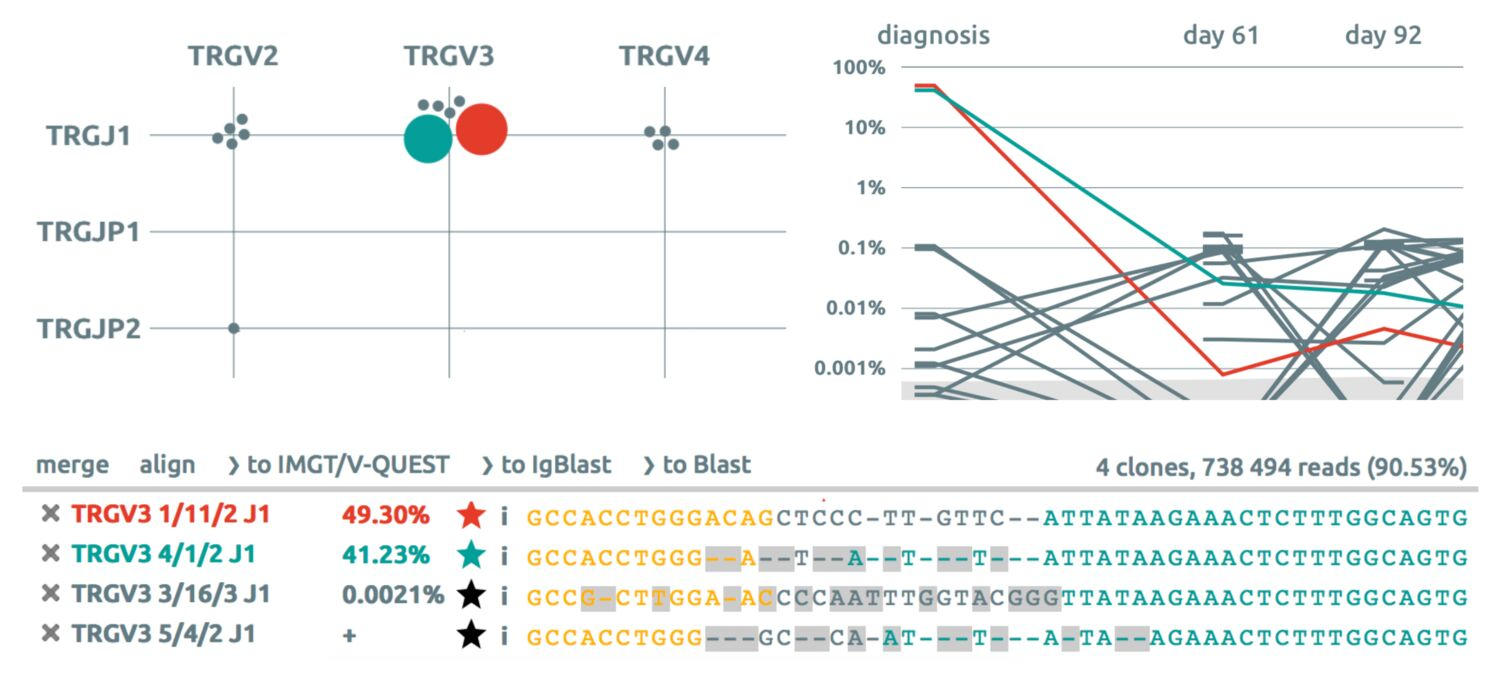
\includegraphics[width=\textwidth]{vidjil-combined.jpg}}

\bigskip

This tutorial is composed of three parts:
the first one about uploading and managing data from several samples on the platform,
and the two last ones about the visualization
part for browsing and analyzing clones one one
or multiple samples.
% (p.~\pageref{sec:part2}) on the usage of multiple samples and on exporting
% data.

You can directly go to the part of the tutorials you are more interested in.
Bear in mind
that the first part of the tutorial uses a dataset that is
provided at the start
while the other parts uses a toy dataset
already available on \texttt{app.vidjil.org}.
% that is provided at the start of the second part.

Main help page of the Vidjil
platform: \url{https://www.vidjil.org/doc/user}


\tableofcontents


\chapter{Part 1 -- Dealing with samples/patients/runs, controlling quality
}

\section{Dealing with samples and patients}
We will see how to make the best use of the patient and sample database and
how to use it efficiently.
For this sake you need an \textit{account} on the public server with the rights to create new patients,
runs, sets, to upload data and, preferably, to run analyses.
Therefore the demo account is not suitable.

\question{ Go to \href{https://app.vidjil.org}{\tt app.vidjil.org} and log in to your account.
You can there click on \com{request an account} if you do not currently have one. 
\marginpar{The public app.vidjil.org server is for test or research use. 
Do not use it for routine clinical data.
The \href{http://www.vidjil.net}{VidjilNet} consortium offers health-certified options for hosting such data.}
}


\question{ Retrieve the toy dataset at
  \href{http://vidjil.org/seqs/tutorial_dataset.zip}{\tt vidjil.org/seqs/tutorial\_dataset.zip}
  and extract the files from the archive.}

You should now have three files. We will imagine that those three files are
the results from a single sequencing run. More precisely, each one corresponds to
a single patient. Thus we now want to upload those files and assign all of
them to a same \com{run} and each of them to a single \com{patient}.

\question{
  Go back to the main page of the Vidjil platform (by default
  \href{https://app.vidjil.org}{\tt app.vidjil.org}).
  You should be on the \com{patients} page.
  Go at the bottom of the page and click on \com{+ new patients} to create the
  three patients.
}
\begin{verbatim}

  cy.goToUsersPage()
  cy.log(`There are ${cy.getTableLength("#table_users")} patients`)
  cy.getTableLength("#table_users").should('be.lt', 20)


\end{verbatim}

Note that usually you should check whether the patient has
already been created by searching her/his name in the search box at the
upper left corner

\question{
  You are now on the  creation page for patients, runs, and sets.
  You can create as many patients, runs and sets as you want.
  \marginpar{Patients, runs and sets are just different ways to
    group samples. 
    The names are just used to add some semantic so that you
    know that your patients will be on the patient page, your runs on the run
    page and your other sets (thus any set of samples you want to make) on the
    run page.}
  Here we already have a line to create one patient.
  We want to create two additional patients and one run.
  Thus click twice on \com{add patient} and once on \com{add run}.
}
\begin{verbatim}
  ///////////////////////////
  cy.log("// test_002_add_new_patient")
    cy.goToPatientPage()
    cy.get('[onclick="db.call(\'sample_set/form\', {\'type\': \'patient\'})"]')
    .click()


\end{verbatim}

  Now you should have three lines with Patient 1, Patient 2, Patient 3 and one
  line with Run 1.
  If you created too many lines you can remove some by clicking on the cross at
  the right hand side.

\question{
  For instance click on the cross corresponding to Patient 3.
  The line has now been removed.
  Click again on \com{add patient} so that the line appears again (it is now
  called Patient 4).
}
\begin{verbatim}
  ///////////////////////////
  cy.log("// test_003_add_new_patient")
    // Add 2 new patients + run lines
    cy.get("#patient_button").click()
    cy.get("#patient_button").click()

    // delete last line
    cy.get(':nth-child(3) > .icon-cancel').click()

    // add another new line
    cy.get("#patient_button").click()

\end{verbatim}

\question{ Now you can fill the mandatory fields (circled with red) and,
  optionally, the other fields.}
\begin{verbatim}
  ////////////////////////////
  cy.log("// test_004_fill_new_patient")
    // Add 2 new patients + run lines
    cy.get('#run_button').click()
    cy.get('#group_select')
      .select("public")
      .trigger("change")


    // Fill forms
    cy.fillPatient(0, "id_p1", "First_name_1", "Last_name_1", "2000-01-01", "")
    cy.fillPatient(1, "id_p2", "First_name_2", "Last_name_2", "2000-01-01", "")
    cy.fillPatient(3, "id_p3", "First_name_3", "Last_name_3", "2000-01-01", "")
    cy.fillRun(0, "id_r1", "run_name 1", "2010-01-01", "run informations #tagtest")
 

\end{verbatim}

The last field is optional but it is very important (the field called
\com{patient/run information (\#tags can be used)}.

Here you can enter any information relevant to this set of samples.
More specifically you can enter tags (starting with a \#) that will allow
you to search very easily and quickly all the patients/runs/sets sharing
this tag.
By default when you enter a \# in this field, some tags appear and the
suggestions are  updated while you enter other characters.
Note that a tag cannot contain any space.
Also note that you can create other tags just by entering whatever you would
like in the field preceded with a \#. Thus any tag you enter is saved (and
can be suggested later on).

\question{For patient 1 in this last field, enter \texttt{\#diagnosis of
    patient with \#B-ALL}. For patient 2, enter \texttt{\#blood sample \#CLL}.
  For patient 4, enter \texttt{bone \#marrow \#B-ALL}}
\begin{verbatim}
  cy.log("// test_005_change_description")
    // Fill forms
    cy.fillPatient(0, "id_p1", "First_name_1", "Last_name_1", "2000-01-01", "#diagnosis of patient with #B-ALL")
    cy.fillPatient(1, "id_p2", "First_name_2", "Last_name_2", "2000-01-01", "#blood sample #CLL")
    cy.fillPatient(3, "id_p3", "First_name_3", "Last_name_3", "2000-01-01", "bone #marrow #B-ALL")

    cy.get('#object_form > .btn')
      .should("have.value", "save")
      .click()

    // land on patient page
    cy.get('tr').contains("Last_name_1 First_name_1 ")
    cy.get('tr').contains("Last_name_2 First_name_2 ")
    cy.get('tr').contains("Last_name_3 First_name_3 ")

\end{verbatim}

\marginpar{{\bf New!}
 Note that patients (and runs and samples) can also be created at once by
pasting a table from a spreadsheet editor. See specification at \href{https://www.vidjil.org/doc/user/\#batch-creation-of-patientsrunssets}{\tt batch-creation-of-patientsrunssets}}

Now the three patients and the run have been created but we have not uploaded
the sequence files yet.

\question{Now go to the \com{runs} page. You should see the run you have just
  created. Click on it. Then click on \com{+ add samples}.}
\begin{verbatim}
  cy.log("// test_006_add_new_run")
    cy.goToRunPage()
    cy.get('tr').contains("run_name 1")
      .click()

\end{verbatim}

Similarly to the patient/run creation page, we can add as many samples as we
want on this page.

\question{As we need to upload three samples, click twice on the \com{add
    other sample} button so that you have three lines to add a sample.}
\begin{verbatim}
  cy.log("// test_007_add_new_samples_line_in_run")
    // Do by the next cypress function call

\end{verbatim}

\question{For sample 1, choose the file corresponding to patient 1 (and
  respectively for patient 2 and 3). You can also add extra information, including
  tags, as previously.}
\begin{verbatim}
  cy.log("// test_008_upload_new_samples_in_run")
    // Do by the next cypress function call

\end{verbatim}

Note the \com{common sets} field. This field means that all the samples will
be added to this run (the one you created). If you would like to \textbf{all}
the samples to another patient/run/set you should specify it here.

In our case we want to add each sample to a different patient. Thus we don't
need to modify this field.

\question{Instead we need to modify the last field on each line. Click on
  it. A list should appear with the last patients/runs/sets you created.
  Either click on the correct patient or type the first letters of her/his
  name. Then validate with \com{Enter} or by clicking on the correct entry.}
\begin{verbatim}
 
  cy.log("// test_009_upload_sample_set_common_sets")
    // Do by the next cypress function call

\end{verbatim}

\question{When you have associated each sample to its corresponding patient
  you can upload the samples by clicking on the \com{Submit samples} button.}
\begin{verbatim}
  cy.log("// test_010_upload_sample_submit")
    var preprocess   = undefined
    var filename1    = "Demo-X5.fa"
    var filename2    = undefined
    var informations = " from tutorial server tests #functional #tutorial"

    cy.addSample(preprocess, "nfs", filename1, filename2, "2010-01-01", "Solo; Sample 1"+informations, "Last_name_1")
    cy.addSample(preprocess, "nfs", filename1, filename2, "2011-01-01", "Solo; Sample 2"+informations, "Last_name_2")
    cy.addSample(preprocess, "nfs", filename1, filename2, "2012-01-01", "Solo; Sample 3"+informations, "Last_name_3")

    var sample_to_add_1 = [preprocess, "nfs", filename1, filename2, "2010-01-01", "Batch; Sample 1x #functional #tutorial; multiple add", "Last_name_1"]
    var sample_to_add_2 = [preprocess, "nfs", filename1, filename2, "2011-01-01", "Batch; Sample 2x #functional #tutorial; multiple add", "Last_name_2"]
    var sample_to_add_3 = [preprocess, "nfs", filename1, filename2, "2012-01-01", "Batch; Sample 3x #functional #tutorial; multiple add", "Last_name_3"]
    cy.multiSamplesAdd([sample_to_add_1, sample_to_add_2, sample_to_add_3])

\end{verbatim}

Now you are back on the page of the run where you should see the three samples
that are being uploaded.

\question{When the upload is finished you launch the analysis by selecting the
configuration in the drop down at the right (\com{multi+inc+xxx}) and then
clicking on the gearwheel.}
\begin{verbatim}
  cy.log("// test_011_launch_analysis_sample")
    var sample_id = 49
    cy.launchProcess("2", sample_id)

\end{verbatim}

You can have a coffee, a tea, or something else, while the process is
launched.

\question{To regularly check the status of your job you can click
  on the \com{reload} button at the bottom left of the page.
  Your process usually goes through the following stages: \com{QUEUED},
  (possibly \com{STOPPED}), \com{RUNNING}, \com{COMPLETED} (or
  \com{FAILED} when there is an issue, in such a case please contact us)}
\begin{verbatim}
  cy.log("// test_012_sample_analysis")
    cy.waitAnalysisCompleted("2", sample_id)

\end{verbatim}

Then you can view the results as explained before.
Instead we will remain on the server.

\question{Now go back to the \com{patients} page. You can filter the page
  using the tags you entered previously.
  Enter \texttt{\#B-ALL} in the search box (notice the autocompletion that helps you)
  and validate with \com{Enter}.}
\begin{verbatim}
  cy.log("// test_013_patient_page_and_filter")
    cy.goToPatientPage()
  
    var value_filter = "#B-ALL"
    cy.dbPageFilter(value_filter)

    cy.get('#db_table_container')
      .find('tbody')
      .find('tr').each(($el, index, $list) => {// $el is a wrapped jQuery element
          // wrap this element so we can use cypress commands on it
          cy.wrap($el).should("contain", value_filter)
    })
    
    var uid_sample2 = 33
    cy.get(`#sample_set_open_${uid_sample2}_config_id_-1`)
      .should("not.exist")

\end{verbatim}


\section{Controlling the quality of a run}

Go to the \com{runs} section, using the button at the top of the page.
For the \textit{Run 1} that you have created at the beginning of this part,
click on the table icon that corresponds to the \textit{Preview/quality
control}.

This offers a global view on the run.

\question{The \com{Clonotypes $\geq 5\,\%$} show the number of clonotypes that
reach a quantification of at least 5\,\% in their own locus. This helps you
identify the polyclonality of a sample.}

\question{When merging reads, you may want to tick the boxes \com{Reads
(merged)} and \com{Pre-process} in order to check the results of the merging
process.}

\question{The \com{Common} column shows the number of clonotypes (above .01\,\%) that are
shared between several samples.}

\question{Hover the plot of the read length distribution. In the first sample
identify the read length of the largest peak by hovering it.}

\question{You can export all this data by clicking on the link at the bottom left.}



\bigskip


\vfill

\centerline{\includegraphics[width=.5\textwidth]{./grid-1}}

\vfill

\newpage ~
\newpage

\chapter{Part 2 --  Browsing and analyzing clones in one sample}

\bigskip



\question{Connect to the public server (\url{https://app.vidjil.org}), either with your account
or the demo account (\texttt{demo@vidjil.org} / \texttt{demo}),
select the \textit{Demo LIL-L3 (tutorial)} patient.
If you don't see it, search for \com{\#Demo} in the top-left search box.
Then click on the bottom right link, \com{see results: multi-inc-xxx}.
Do not open the \textit{Demo LIL-L3 (analyzed)} patient: this one contains the complete
analysis.
The Vidjil web application opens.}

This patient (patient 063 from \href{http://dx.doi.org/10.1016/j.leukres.2016.11com.009}{Lille study on the feasibility of MRD using HTS}) suffering T-ALL has one diagnosis sample,
with dominant clones both in IGH and TRG,
and four follow-up samples, including a relapse.

\question{In the \com{settings} menu, try the various options for \com{sample key}.
  The five samples can be labeled by their name, their date of sampling or by the number of days after the first sample.
}

In the following sections, we focus on the diagnosis sample.
% and explore how to assess the quality of the data
% how to view and filter clones and
The section~\ref{sec:tracking} will deal with the comparison of several samples. 



\section{Assessing the quality of the run and of the analysis}
\begin{verbatim}


  // ########################################################
  // ### Assessing the quality of the run and of the analysis
  // ########################################################

\end{verbatim}

The Vidjil web application allows to run several ``AIRR/RepSeq'' (immune repertoire analysis) algorithms.
Each AIRR/RepSeq algorithm has its own definition of what a clone is (or, more precisely
a clonotype), how to output its sequence and how to assign a V(D)J designation.
The number of analyzed reads will depend on the algorithm used.
This sample has been processed using the Vidjil algorithm.


\marginpar{The percentage of analyzed reads can range from .01\,\% or below (for
  RNA-Seq or capture data) to 98-99\,\% or above (for amplicon libraries with high-quality runs).}
\question{How many reads have been analyzed in the current sample by Vidjil-algo?}
\reponse{In the upper left corner, you can see an information panel with \com{analyzed reads 1 967 338 (82.31\,\%)'}}
\begin{verbatim}

  cy.log("// test_A_quality_01_number_reads")
  cy.get('#info_segmented').contains("1 967 338 (82.31%)")
  cy.get('#info_selected_locus').contains("1 965 646 (82.24%)")

\end{verbatim}

Now we will try to assess the reason why some reads were not analyzed in our
sample.
This might reflect a problem during the sequencing protocol\dots or that could
be normal.
For that sake you will need to display the information box by clicking on the
\textit{i} in the upper left part.
\question{What are the average read lengths on IGH? and on TRG?}

\reponse{In the Analysis log row, under \com{av. len}\\*
IGH \fl 314.5\\*
TRG \fl 197.6 }
\begin{verbatim}

    cy.log("// test_A_quality_02_sample_log")
    cy.get('.button > .icon-info').click()
    cy.get('#modal_line_title_info_timepoint_reads').should("be.visible")

    cy.get('#modal_line_value_info_timepoint_reads').contains('2390273')
    cy.get('#modal_line_value_info_timepoint_analyzed_reads').contains('1967338')
    cy.get('#modal_line_value_info_timepoint_log').contains('IGH               ->   562520   314.5      31770   0.056')
    cy.get('#modal_line_value_info_timepoint_log').contains('TRG               ->  1403126   197.6      73089   0.052')
    cy.get('#modal_line_value_info_timepoint_log').contains('UNSEG only V/5\'   ->   332125   191.2')


    cy.get('.data-container > .closeButton > .icon-cancel').click()
    cy.get('#info_timepoint').should("not.exist")


\end{verbatim}

The lines starting with \texttt{UNSEG} display the reasons why some reads have
not been analyzed.

You can see what those reasons mean in the online documentation of the
algorithm:

 \centerline{\tt\href{http://www.vidjil.org/doc/vidjil-algo/\#reads-without-detected-recombinations}{vidjil.org/doc/vidjil-algo\#reads-without-detected-recombinations}}

\question{What are the major causes explaining the reads have not been
  analyzed? Also have a look at the average read lengths of these causes. Do
  you notice something regarding the average read lengths?}


\reponse{ 1. The algorythm was not able to find a V or a J for most of the unsegmeneted reads.\\*
2. The may be too short to cover enough of the V or J genes to be detected. }

\section{Viewing and filtering clones}


\subsection{Looking at a clone}
\begin{verbatim}


  #################################
  ### Viewing and filtering clones
  #################################

\end{verbatim}

Each RepSeq algorithm has its own definition of what a clone is (or, more precisely
a clonotype), and on how to output its sequence and how to assign a V(D)J designation.

In this file, the most abundant clone
is \texttt{IGHV3-9 7/CCCGGA/17 J6*02}.

\question{Select this clone, either by clicking on the list or on the grid.
  How many reads do this clone represent? (see again the bottom part to the right)}

\reponse{The bottom panel display information about currently selected clones \fl 189 991 reads (9.665\,\%)}

\begin{verbatim}
  def test_B_clones_01_major
    # major clone of sample 0 is clone 1 
    clone = $b.clone_in_list("1").click
    cinfo = $b.clone_info("1")
    assert ( cinfo[:name].text == "IGHV3-9 7/CCCGGA/17 J6*02"), "correct name for first clone"

    stats = $b.statsline
    assert (stats.text.include? '1 clonotype, 189 991 reads (9.665%)'),  "Correct stats, number of reads and percentage: " + stats.text
  end
\end{verbatim}


There are several options to display the V(D)J designation.

\question{In the  \com{settings} menu, under \com{N regions in clonotype names} select \com{length} to show N zones by their length. Revert to the
  default \com{sequence (when short)} setting to show the full N on short sequences.}

\begin{verbatim}
  def test_B_clones_02_setting_n_length
    $b.menu_settings.click
    $b.input(:id => "menuCloneNot_nucleotide_number").click
    $b.update_icon.wait_while(&:present?) # wait update
    cinfo = $b.clone_info("1")
    assert ( cinfo[:name].text == "IGHV3-9 7/6/17 J6*02"), "correct name for first clone (nucleotide_number)"
    cinfo30 = $b.clone_info("30")
    assert ( cinfo30[:name].text == "IGHV3-13*05 1/55/16 J6*02"), "correct name for 30th clone (nucleotide_number)"

    $b.menu_settings.click
    $b.input(:id => "menuCloneNot_short_sequence").click
    $b.update_icon.wait_while(&:present?) # wait update
    cinfo = $b.clone_info("1")
    assert ( cinfo[:name].text == "IGHV3-9 7/CCCGGA/17 J6*02"), "correct name for first clone (short_sequence)"
    cinfo30 = $b.clone_info("30")
    assert ( cinfo30[:name].text == "IGHV3-13*05 1/55/16 J6*02"), "correct name for 30th clone (short_sequence)"

    $b.menu_settings.click
    $b.input(:id => "menuCloneNot_full_sequence").click
    $b.update_icon.wait_while(&:present?) # wait update
    cinfo = $b.clone_info("1")
    assert ( cinfo[:name].text == "IGHV3-9 7/CCCGGA/17 J6*02"), "correct name for first clone (full_sequence)"
    cinfo30 = $b.clone_info("30")
    assert ( cinfo30[:name].text == "IGHV3-13*05 1/GAGGGGGGCCTCCCTCCACCCCTCTAACCAGTGAAAAGCAAACTGGGCCCAGCGG/16 J6*02"), "correct name for 30th clone (full_sequence)"

    # Reset params as nucleotide number
    $b.menu_settings.click
    $b.input(:id => "menuCloneNot_nucleotide_number").click
    $b.update_icon.wait_while(&:present?) # wait update
  end
\end{verbatim}

\question{Try also the options  \com{alleles in clonotype names} : by selecting \com{always}, the clone
  V gene is displayed as \com{IGHV3-9*01}. Revert to the default \com{when not
    *01}. This setting, which is the default, allows to have a more condensed
  V(D)J designation that doesn't make the \com{*01} appear (it is implicit).}


\begin{verbatim}
  def test_B_clones_03_setting_allele
    $b.menu_settings.click
    $b.input(:id => "menuAlleleNot_never").click
    $b.update_icon.wait_while(&:present?) # wait update
    cinfo = $b.clone_info("1")
    assert ( cinfo[:name].text == "IGHV3-9 7/6/17 J6"), "correct name for first clone (menuAlleleNot_never): " + cinfo[:name].text

    $b.menu_settings.click
    $b.input(:id => "menuAlleleNot_when_not_01").click
    $b.update_icon.wait_while(&:present?) # wait update
    cinfo = $b.clone_info("1")
    assert ( cinfo[:name].text == "IGHV3-9 7/6/17 J6*02"), "correct name for first clone (menuAlleleNot_when_not_01)"

    $b.menu_settings.click
    $b.input(:id => "menuAlleleNot_always").click
    $b.update_icon.wait_while(&:present?) # wait update
    cinfo = $b.clone_info("1")
    assert ( cinfo[:name].text == "IGHV3-9*01 7/6/17 J6*02"), "correct name for first clone (menuAlleleNot_always)"

  end
\end{verbatim}

\subsection{Showing more clones}

By default Vidjil displays the 50 most abundant clones at each time point.
With five time points, we may therefore have from 50 to 250 clones displayed
depending if the top 50 are always the same or always different or, more
realistically, in-between.
This number can be increased to a maximum of 100 clones by going to the \com{filter} menu and by putting the
slider to its right end.
\question{Notice how the IGH smaller clonotypes percentage (second clone displayed in the list) changes. What was its
  initial value? What is it now?}

\reponse{filter set to 50 \fl IGH smaller clonotypes 10.11\,\%\\*
 filter set to 100 \fl IGH smaller clonotypes 8.92\,\%\\*}
\begin{verbatim}
  def test_B_clones_04_filter_slider
    if not ENV['HEADLESS']
      # Igh small position: 454
      cinfo = $b.clone_info("454")
      assert ( cinfo[:size].text == "10.11%"), "correct name for first clone (short_sequence)"

      ## Change slider value
      assert ( not $b.clone_in_list('308').present?), "small clone is not present in list (before slider increase)"
      slider = $b.menu_item("top_slider")
      slider.click
      $b.menu_filter.hover
      slider.send_keys :arrow_right 
      slider.send_keys :arrow_right
      slider.send_keys :arrow_right
      $b.clone_in_list("0").click
      ### exist in scatterplot
      $b.clone_in_list('308').wait_until(&:present?) # "small clone is present in list (after slider increase)"
      assert ( not $b.clone_in_list('309').present?), "Not all real clones are present in list"

      ## control by size of smaller clone
      assert ( cinfo[:size].text == "9.768%"), "correct name for first clone (short_sequence)"

      ### decrease by slider usage
      slider = $b.menu_item("top_slider")
      slider.click
      $b.menu_filter.hover
      slider.send_keys :arrow_left 
      $b.clone_in_list("0").click
      $b.update_icon.wait_while(&:present?)

      ### exist in scatterplot
      assert ( not $b.clone_in_list('308').present?), "a small clone is hidden if slider decrease"
      assert ( cinfo[:size].text == "10.11%"), "correct name for first clone (short_sequence) after decrease slider value"
    end
  end
\end{verbatim}

The \textit{smaller clonotypes} correspond to clones that are not displayed
because they are never among the most abundant ones.


\subsection{Tagging and filtering clones}

Consider the most abundant clones in the list:  \texttt{IGHV3-9 7/CCCGGA/17 J6*02} and  \texttt{TRGV10 13//5 JP1}.
Usually we may want to tag them in order to remember them later on.
\question{Click on the star and choose colored tags for these two clones, such as \texttt{clonotype 1} or \texttt{clonotype 2}.
  Notice how the color applies throughout all the views.}

\begin{verbatim}
  def test_B_clones_05_tag_biggest_clone
    # control default color of clones
    assert ($b.clone_info('0')[:name].style('color') ==  'rgba(101, 123, 131, 1)' )

    $b.clone_in_list("0").click
    $b.clone_info("1")[:star].click # top IGH
    $b.tag_item('0')[:name].click
    $b.clone_info("4")[:star].click # top TRG 
    $b.tag_item('1')[:name].click
    $b.clone_info("0")[:star].click ## clone rechute
    $b.tag_item('4')[:name].click
    $b.update_icon.wait_while(&:present?)
    $b.clone_in_list("5").click ## select other clone to see real color of clone 0

    # New color
    assert ($b.clone_info('0')[:name].style('color') ==  'rgba(108, 113, 196, 1)' )
  end
\end{verbatim}

Later you may want to filter clones depending on the tags you have chosen.

\question{In the upper left part, click on the little dark gray square (the
  second coloured square starting from the right). What happens? What if you click again?}

\begin{verbatim}
  def test_B_clones_06_filter_by_tag
    assert ($b.clone_in_list("1").present?), "clone 0 is present at starting test"

    # Click on tag switch; clone 1 will be hidden
    $b.info_colorBy.span(title: 'clonotype 1').click
    $b.update_icon.wait_while(&:present?)
    assert (not $b.clone_in_list("1").present?), "clone 0 is hidden"

    $b.info_colorBy.span(title: 'clonotype 1').click
    $b.update_icon.wait_while(&:present?)
    assert ($b.clone_in_list("1").present?), "clone 0 is present at the end of the test"
  end
\end{verbatim}

This is a way of filtering some clones. This may be useful when we want to
focus on some specific clones. Another way of doing so is to filter them by
their gene names or by their DNA sequences.  
\question{In the search box,
  enter \texttt{GGAGTCGGGG} and validate with \texttt{Enter}.  How many sequences are
  left?}


\begin{verbatim}
  def test_B_clones_06b_filter_by_tag
    # TODO
  end
\end{verbatim}

Note that the search is performed both on the forward and the reverse strand.
\question{Check that by searching for the reverse complement of the
  sequence: \texttt{CCCCGACTCC}. Do you find the same results as previously?}
\question{How can you cancel this filter and view again all the clones?}

\begin{verbatim}
  def test_B_clones_07_filter_search_area
    ## test that clone are present before filtering
    assert ( $b.clone_in_list('0').present?),  ">> clone 0 is present"
    assert ( $b.clone_in_list('1').present?),  ">> clone 1 is present"
    #assert ( $b.clone_in_list('212').present?),  ">> clone 212 is present"
    assert ( $b.clone_in_list('454').present?),  ">> clone 454 is present"

    filter = $b.filter_area
    filter.value = 'CCCCGACTCC'
    $b.send_keys :enter
    $b.update_icon.wait_while(&:present?)
    # clone present before filtering; not after
    assert ( not $b.clone_in_list('0').present?), ">> clone 0 is hidden"
    assert ( not $b.clone_in_list('1').present?), ">> clone 1 is hidden"
    #assert ( not $b.clone_in_list('212').present?), ">> clone 212 is hidden"
    assert ( not $b.clone_in_list('454').present?), ">> clone 454 is hidden"
    # clones that should stay present (19 clones, test somes)
    assert (     $b.clone_in_list('6').present?),   ">> clone 6   is present even with filtering"
    assert (     $b.clone_in_list('142').present?), ">> clone 142 is present even with filtering"
    assert (     $b.clone_in_list('51').present?),  ">> clone 51  is present even with filtering"
    assert (     $b.clone_in_list('52').present?),  ">> clone 52  is present even with filtering"
    assert (     $b.clone_in_list('16').present?),  ">> clone 16  is present even with filtering"

    # tester le nombre de clone présents

    $b.clear_filter.click
    $b.clone_in_scatterplot('1').hover
    ## test that clone are present again after remove filter
    assert ( $b.clone_in_list('0').present?),   ">> clone 0 is present again"
    assert ( $b.clone_in_list('1').present?),   ">> clone 1 is present again"
    #assert ( $b.clone_in_list('212').present?), ">> clone 212 is present again"
    assert ( $b.clone_in_list('454').present?), ">> clone 454 is present again"
  end
\end{verbatim}  
\bigskip

Another solution to tag a specific clone is to rename it.
\question{Double click on the name of a clone (in the list of clones) and
  choose another name (\textit{e.g.} interesting clone) and validate using
  \texttt{Enter}.}
\begin{verbatim}
  def test_B_clones_08_change_clone_name
    $b.clone_in_list("1").click
    cinfo = $b.clone_info("1")
    cinfo[:name].double_click # set mode to allow setting

    $b.clone_name_editor.set 'interesting clone'
    $b.clone_name_saver.click
    $b.update_icon.wait_while(&:present?)
    assert (cinfo[:name].text == 'interesting clone'), " >> clone name ('interesting clone') has changed"
  end
\end{verbatim}

\bigskip

After this rename, you can see that the clone is still selected.
\question{Click on several clones by holding the \texttt{Ctrl} key to select
  more. Each time you add a new clone to the selection, its sequence
  is added in the bottom part.}
\begin{verbatim}
  def test_B_clones_09_multiselection
    $b.menu_filter.click
    $b.update_icon.wait_while(&:present?)
    $b.send_keys 4
    $b.update_icon.wait_while(&:present?)
    # to verify correct selection, We will look in segmenter the presence if clone entrie
    # Maybe another method could be more acurate
    
    $b.clone_in_list("1").click
    $b.update_icon.wait_while(&:present?)
    assert ( not $b.clone_in_segmenter('0').present? ), ">> Another click; Clone 0 should not be present anymore in segmenter"
    assert (     $b.clone_in_segmenter('1').present? ), ">> Another click; Correct selection of clone 1 after second click in scatterplot"
   
    $b.clone_in_list("0").click(:control)
    $b.update_icon.wait_while(&:present?)
    # clone is present in segmenter
    assert ( $b.clone_in_segmenter('0').present? ), ">> ctrl+click; Clone 0 should be present in segmenter"
    assert ( $b.clone_in_segmenter('1').present? ), ">> ctrl+click; Clone 1 should be present in segmenter"
    # As whell than their sequences ? TODO
  end
\end{verbatim}

\question{How many clones are selected? How many reads do those clones
  represent?}
\begin{verbatim}
  def test_B_clones_10_size_if_multiple_selection
    $b.clone_in_list("1").click
    $b.clone_in_list("4").click(:control)
    $b.update_icon.wait_while(&:present?)

    stats = $b.statsline
    assert (stats.text.include? '2 clonotypes, 364 027 reads (18.51%)'),  "Correct stats, number of reads and percentage"
  end
\end{verbatim}

\question{ Notice the star at the the right of the screen, near the number
  of reads. You can also tag clones using this icon. In that way, you will be able to tag
  all the selected clones at once.}
\begin{verbatim}
  def test_B_clones_11_multiple_tag
    $b.clone_in_list("7").click
    $b.clone_in_list("11").click(:control)
    $b.clone_in_list("13").click(:control)
    $b.update_icon.wait_while(&:present?)

    $b.element(:id => "tag_icon__multiple").click
    $b.element(:id => 'tagElem_6').click
    $b.update_icon.wait_while(&:present?)
    $b.clone_in_list("0").click(:control) # select another clone, else last selected still keep default color as "hover"
    assert ($b.clone_info('5')[:name].style('color') ==  'rgba(101, 123, 131, 1)' ) , "clone 5 still have default color"
    assert ($b.clone_info('7')[:name].style('color') ==  'rgba(211, 54, 130, 1)' ) , "clone 7 have also changed color"
    assert ($b.clone_info('11')[:name].style('color') ==  'rgba(211, 54, 130, 1)' ) , "clone 11 have also changed color"
    assert ($b.clone_info('13')[:name].style('color') ==  'rgba(211, 54, 130, 1)' ) , "clone 13 have also changed color"
  end
\end{verbatim}

\question{When you want to focus on the selected clones, you can click on the
  focus link on the right, next to the number of selected clones.
  This feature is useful when you want to analyse some clones more thoroughly
  without being annoyed by other clones.}
\begin{verbatim}
  def test_B_clones_12_focus
    ## test that clone are present before focus
    assert ( $b.clone_in_list('1').present?), ">> clone 1 is present"
    assert ( $b.clone_in_list('7').present?), ">> clone 7 is present"
    assert ( $b.clone_in_list('11').present?), ">> clone 11 is present"
    
    # select somme clones (7, 11, 13)
    $b.clone_in_list("7").click
    $b.clone_in_list("11").click(:control)
    $b.clone_in_list("13").click(:control)
    $b.update_icon.wait_while(&:present?)
    $b.span(:id => "focus_selected").click
    $b.update_icon.wait_while(&:present?)

    ## test that clone are hidden after focus
    assert ( not $b.clone_in_list('1').present?), ">> clone 1 is hidden"
    assert (     $b.clone_in_list('7').present?), ">> clone 7 is present"
    assert (     $b.clone_in_list('11').present?), ">> clone 3 is present"
    assert ( not $b.clone_in_list('5').present?), ">> clone 5 is hidden"
  end
\end{verbatim}

\question{To remove this focus, click on the cross next to the search box,
  above the list.}
\begin{verbatim}
  def test_B_clones_13_remove_filter
    ## test that clone are present after resetting filtering
    $b.span(:id => "reset_focus").click
    $b.update_icon.wait_while(&:present?)
    assert ( $b.clone_in_list('1').present?), ">> clone 1 is present again"
    assert ( $b.clone_in_list('7').present?), ">> clone 7 is still present"
    assert ( $b.clone_in_list('5').present?), ">> clone 5 is present again"
  end
\end{verbatim}

\question{To unselect them all, you can click in an empty area on the top or
  bottom plot.}
\begin{verbatim}
  def test_B_clones_14_unselect_by_click_in_empty_zone
    # TODO
  end
\end{verbatim}

Sometimes, one wants to hide noisy or unrelated clones.

\question{Select a clone or several clones and click on the \com{hide} button, near the \com{focus} button. Show again these
  clones by clicking on the cross next to the search box.}
\begin{verbatim}
  def test_B_clones_15_hide_selected
    ## test that clone are present before focus
    assert ( $b.clone_in_list('1').present?), ">> clone 1 is present"
    assert ( $b.clone_in_list('7').present?), ">> clone 7 is present"
    assert ( $b.clone_in_list('11').present?), ">> clone 11 is present"
    
    # select somme clones (7, 11, 13)
    $b.clone_in_list("7").click
    $b.clone_in_list("11").click(:control)
    $b.clone_in_list("13").click(:control)
    $b.update_icon.wait_while(&:present?)
    $b.span(:id => "hide_selected").click
    $b.update_icon.wait_while(&:present?)

    ## test that clone are hidden after focus
    assert (     $b.clone_in_list('1').present?), ">> clone 1 is present"
    assert ( not $b.clone_in_list('7').present?), ">> clone 7 is hidden"
    assert ( not $b.clone_in_list('11').present?), ">> clone 3 is hidden"
    assert (     $b.clone_in_list('5').present?), ">> clone 5 is present"

    ## test that clone are present after resetting filtering
    $b.span(:id => "reset_focus").click
    $b.update_icon.wait_while(&:present?)
    assert ( $b.clone_in_list('1').present?), ">> clone 1 is present again"
    assert ( $b.clone_in_list('7').present?), ">> clone 7 is still present"
    assert ( $b.clone_in_list('5').present?), ">> clone 5 is present again"

    ## test that clone are present after resetting filtering
    $b.clear_filter.click
    $b.update_icon.wait_while(&:present?)
    assert ( $b.clone_in_list('1').present?), ">> clone 1 is present again"
    assert ( $b.clone_in_list('7').present?), ">> clone 7 is still present"
    assert ( $b.clone_in_list('5').present?), ">> clone 5 is present again"
  end
\end{verbatim}

% Another way to hide clonesis to assign is to change the tag of it as ``standard (niose)`` and choose to uncheck this tag by clicking on the corresponding tile on the list of tiles at the informatons panel to switch them from a visible state to a filter one.
%%% Voir ci-dessus, déjà mis

It is also possible to filter samples that do not contain a clone.  When you
have lots of samples it helps to keep the sample of interest.  Here the number
of sample is quite limited, so the feature may appear less useful.

\question{\new Click on the \com{IGHV3-11 / IGHJ6} clone in the last sample, whose
  abundance is around 10\,\%.
  Then go in the menu at the upper-right corner of the graph (where \com{5/5}
  is written) and select \com{focus on selected clones}.
}
\begin{verbatim}
  def test_B_clones_16_graphmenu_filter
    assert ( $b.clone_in_list('5').present?), ">> clone 5 is present again"
    div_ratio = $b.span(:id => "visu2_title")
    assert ( div_ratio.text == "5 / 5" ), "Ratio show is correct at init"
    time0 = $b.graph_x_legend("0")
    check0 = $b.checkbox(:id => "visu2_listElem_check_0")
    check2 = $b.checkbox(:id => "visu2_listElem_check_2")
    assert ( time0.present? ), "first sample is present in timeline"
    assert ( check0.set? ), "first checkbox is true"
    assert ( check2.set? ), "third checkbox is true"

    $b.clone_in_list("5").click
    $b.update_icon.wait_while(&:present?) # wait update
    $b.div(:id => 'visu2_menu').hover
    $b.table(:id => "visu2_table").wait_until(&:present?)
    $b.td(:id => 'visu2_listElem_hideNotShare').click
    $b.update_icon.wait_while(&:present?) # wait update

    assert ( div_ratio.text == "3 / 5" ), "Ratio show is correct after focus"
    assert ( not time0.present? ), "first sample is hidden in timeline menu"
    assert ( not check0.set? ), "first checkbox is false"
    assert ( check2.set? ), "third checkbox is true"
  end
\end{verbatim}

By selecting this, the samples where this clone doesn't appear are hidden.
This is useful for instance to assess the contamination among dozens of
samples.

\question{You can go back to the previous view by returning into the menu and
  clicking on \com{show all}. Notice also how in the menu you can select the
  samples to be shown.}
\begin{verbatim}
  def test_B_clones_17_graphmenu_activate
    time0 = $b.graph_x_legend("0")
    check0 = $b.checkbox(:id => "visu2_listElem_check_0")
    check1 = $b.checkbox(:id => "visu2_listElem_check_1")
    check2 = $b.checkbox(:id => "visu2_listElem_check_2")
    div_ratio = $b.span(:id => "visu2_title")
    
    ### starting state
    assert ( div_ratio.text == "3 / 5" ), "Ratio show is correct after focus"
    assert ( not check0.set? ), "first checkbox is false"
    assert ( check2.set? ), "third checkbox is true"

    ### Switch the first sample only (by checkbox)
    $b.div(:id => 'visu2_menu').hover
    $b.table(:id => "visu2_table").wait_until(&:present?)
    check0.click
    $b.until { time0.present? }  # Test "first sample is NOT present in timeline after click"
    assert ( check0.set? ), "first checkbox is true"
    assert ( div_ratio.text == "4 / 5" ), "Ratio show is correct at init"

    ### Click on show all
    $b.td(:id => 'visu2_listElem_showAll').click
    $b.update_icon.wait_while(&:present?) # wait update

    assert ( div_ratio.text == "5 / 5" ), "Ratio show is correct at init"
    assert ( check0.set? ), "first checkbox is true"
    assert ( check1.set? ), "second checkbox is true"
    assert ( check2.set? ), "third checkbox is true"
  end
\end{verbatim}

\section{Analysing clone populations}

\subsection{Clustering clones through inspection of their sequences}

The first thing to be done is to see if some clones should be clustered (because
of sequencing or PCR errors for instance). This step could be automatized
but, in any case, the automatic clustering would need to be checked by an expert
eye.

By default in the bottom plot (the \textit{grid}), the clones
  are displayed according to their V and J genes (or more generally to their
  5' and 3' genes). 

\question{Identify in the grid the clones with an
  \textit{IGHV-3-13}~\textit{IGHJ6} recombination and select them
  all. You can do so either by holding \texttt{Ctrl} or by drawing a rectangle around the clones while
  maintaining down the left button of the mouse.}
\begin{verbatim}
  def test_B_clones_18_select_mulitple_ighv3_13_clonotype
    $b.clone_in_list("0").click
    $b.send_keys 0

    $b.scatterplot_x_legend(8).click # clonotype with IGHV3-13

    ## control that these clonotype is selected and visible in semgenter
    assert ( not $b.clone_in_segmenter('0').present? ), "clone 0 chould not be present";
    assert (     $b.clone_in_segmenter('30').present? ), "clone 30/A should be present";
    assert (     $b.clone_in_segmenter('43').present? ), "clone 43/B should be present";
    assert (     $b.clone_in_segmenter('47').present? ), "clone 43/C should be present";

  end
\end{verbatim}

The sequences of the clones now appear in the bottom part of the browser (the
\textit{sequence panel}). If many clones are selected you can view more sequences
by moving the mouse above the sequence panel.
 In such a case, you may be bothered by the sequence panel going up and
down each time your mouse enters or exits the sequence panel. You can stick it
in its current shape by clicking on the pin at the upper right corner of the
sequence panel.

Then, the sequences in the sequence panel can be visually compared but you can also align
them to see more easily their similarities.


\question{Click on the \com{align} button on the left-hand side. The differences are
emphasized in bold.}
\begin{verbatim}
  def test_B_clones_19_align
    # TODO; align don't available without server
  end
\end{verbatim}

Now it is the user's expertise to determine if sequences are sufficiently
similar, depending on her or his specific question. If some sequences don't appear to be similar enough, you can remove
them from the sequence panel by clicking on the cross in front of the sequence in
the sequence panel.
\question{Remove all the sequences that are not similar enough with the first
  one.}
\begin{verbatim}
  def test_B_clones_20_unselect_from_segmenter
    $b.clone_in_segmenter("47").i(:class => "icon-cancel").click
    $b.update_icon.wait_while(&:present?)
    assert ( not $b.clone_in_segmenter('47').present? ), "clone 47/C should be present";
  end
\end{verbatim}

Now all the sequences in the sequence panel should be highly similar. All their
differences could be due to sequencing or PCR errors.
These artifacts (mutations, homopolymers, insertions, deletions)
depend on the sequencer and the PCR technique.

\question{Cluster all those clones in a single clone by clicking on the ``cluster''
  button, next to the \com{align} button.}
\begin{verbatim}
  def test_B_clones_21_click_on_merge
    $b.merge.click
    $b.update_icon.wait_while(&:present?)

    assert (     $b.clone_in_list("30").present? ),  ">> Real clone A should be present in list "
    assert ( not $b.clone_in_list("43").present? ),  ">> Real clone B should NOT be present in list (clustered)"
    assert (     $b.clone_in_list("47").present? ),  ">> Real clone C should be present in list (not present in segmenter when merged)"
  end
\end{verbatim}

All the clustered sequences now appear within a same clone. That can be seen
in the list: the clone which hosts the subclones appears with a $+$ on its
left. You can click on the $+$ to see the subclones that have been clustered in
the main one.
\question{Click on the $+$ and observe the changes in the grid.}
\begin{verbatim}
  def test_B_clones_22
    # TODO
  end
\end{verbatim}

As you may have noticed the subclones appear again in the grid. You can
compare their sequences again if you'd like (for example to double check that
you were right to cluster them). You can also remove some subclones from the
cluster by clicking on the cross at their left in the list.
\question{For the sake of the exercise, remove the last clone of the cluster.}
\begin{verbatim}
  def test_B_clones_23
    # TODO
  end
\end{verbatim}

\question{%
%For the next step, choose the preset \com{V distribution} (keyboard shortcut \com{5}).
% On n'a pas encore parlé ici des presets. 
Open the \com{cluster} menu, and choose \com{cluster by V/5}. What happened ? There are now two clones with TRGV2. Why ?}
%%  Confirm this by changing the x axis into ``V allele``.
%%% -> Problème, on n'a pas encore parlé des axes à cet endroit.
\begin{verbatim}
  def test_B_clones_24_cluster_by_V
    $b.element(:id => "cluster_menu").hover
    $b.element(:id => "clusterBy_5").wait_until(&:present?)
    $b.element(:id => "clusterBy_5").click

    ## TODO; wait MR !811
  end
\end{verbatim}

\question{In the \com{cluster} menu, select  \com{revert to previous clusters} to undo these clusterings.}
\begin{verbatim}
  def test_B_clones_25
    $b.element(:id => "cluster_menu").hover
    $b.element(:id => "cluster_break_all").wait_until(&:present?)
    $b.element(:id => "cluster_break_all").click
    ## TODO; wait MR !811
  end
\end{verbatim}

\subsection{Other metrics and analysis on the clones}

As a proxy to sequence similarity we used the V and J genes, however there are
other ways to assess sequence similarity that may be more pertinent.
Moreover you may want to plot other metrics on the lymphocyte population.
%
For instance we can choose to plot the V genes versus the length of the N
insertions.
\question{Go to the \com{plot} menu (in the upper left corner of the grid),
  and in the preset box choose \com{V/N length}.}
\begin{verbatim}
  def test_B_clones_26_change_scatter_axis
    # change preset, first time manually as user can do (don't use $b.scatterplot_select_preset this time) 
    select_preset = $b.select_list(:name => "select_preset[]")
    $b.element(:id => "visu_sp_menu").hover
    select_preset.select("V/N length")
    $b.update_icon.wait_while(&:present?)

    assert ( $b.scatterplot_x_label.text == "V/5' gene" ), "Correct legend for axe X for preset V/N length"
    assert ( $b.scatterplot_y_label.text == "N length" ), "Correct legend for axe Y for preset V/N length"
    assert ( $b.scatterplot_x_legend(0).text == "IGHV1-2"), "scatterplot_legend X for this preset is 'IGHV1-2'"
    assert ( $b.scatterplot_y_legend(0).text == "?"), "scatterplot_legend Y for this preset is '0'"
  end
\end{verbatim}

Then you can continue aligning and clustering clones if necessary.

\question{You can also try the preset \com{read length/GC content}
  which tends to separate quite nicely the distinct clones.}
\begin{verbatim}
  def test_B_clones_27_change_preset_2
    $b.scatterplot_select_preset "read length / GC content"
    $b.update_icon.wait_while(&:present?)

    assert ( $b.scatterplot_x_label.text == "Reads length" ), "Correct legend for axe X for preset 0"
    assert ( $b.scatterplot_y_label.text == "GC content" ), "Correct legend for axe Y for preset 0"
    $b.update_icon.wait_while(&:present?)
    assert ( $b.scatterplot_x_legend(0).text == "?"), "scatterplot_legend X pos 0 for this preset is '?'"
  end
\end{verbatim}

Note that you can choose any axis to be plotted: just go the \com{plot} menu and
select any value you would like for the $x$ axis and for the $y$ axis.
For bar charts, the box sizes always relates to the clone size,
and the $y$ axis selects the order of the boxes sharing a same $x$).

%% \item Regarder les stats disponibles, mettre n°7 (taille des reads)

\question{In the \com{plot} menu, switch between the ``bubble plot'' and the ``bar plot''.
In the bar plot mode, pass the mouse over the bars: What happens?}
\begin{verbatim}
  def test_B_clones_28_switch_scatterplot_mode

    skip_on_browser('firefox', '32.0', 'See issue #4595')

    $b.send_keys 0
    $b.update_icon.wait_while(&:present?)
    assert ( $b.scatterplot_x_label.text == "V/5' gene" ), "Correct legend for axe X for preset 0"
    assert ( $b.scatterplot_y_label.text == "J/3' gene" ), "Correct legend for axe Y for preset 0"

    $b.element(:id => "visu_sp_menu").hover
    $b.div(:id => "visu_bar").click
    $b.update_icon.wait_while(&:present?)
    assert ( $b.scatterplot_x_label.text == "V/5' gene" ), "Correct legend for axe X after switch in bar mode"
    assert ( $b.scatterplot_y_label.text == "Size" ), "Correct legend for axe Y after switch in bar mode"

    $b.element(:id => "visu_sp_menu").hover
    $b.div(:id => "visu_plot").click
    $b.update_icon.wait_while(&:present?)
    assert ( $b.scatterplot_x_label.text == "V/5' gene" ), "Correct legend for axe X after switch back in bubble mode"
    assert ( $b.scatterplot_y_label.text == "J/3' gene" ), "Correct legend for axe Y after switch back in bubble mode"
  end
\end{verbatim}

% Another possibility is to request Vidjil to compute the similarity between
% clones.
% \question{Now select the preset \com{plot by similarity} or even \com{plot
%   similarity by locus} to plot similarity for the current locus (beware: this
% may take some time).}
% Now the most similar clones should be close together. However note that it is
% theoretically impossible to achieve such a representation in 2 dimensions. So
% it is possible that two dissimilar clones are close together or, conversely,
% that two similar clones are far apart.

\question{Press the keys \texttt{0} to \texttt{9} on the numeric keypad. What happens ?}
\begin{verbatim}
  def test_B_clones_29_shortcut_preset

    skip_on_browser('firefox', '32.0', 'See issue #4595')

    $b.send_keys 0
    $b.update_icon.wait_while(&:present?)

    assert ( $b.scatterplot_x_label.text == "V/5' gene" ), "Correct legend for axe X for preset 0"
    assert ( $b.scatterplot_y_label.text == "J/3' gene" ), "Correct legend for axe Y for preset 0"
    # assert ( $b.scatterplot_x_legend(0).text == "IGHV1-2"), "scatterplot_legend X at init; IGHV1-2"
    # assert ( $b.scatterplot_y_legend(0).text == "IGHJ1"), "scatterplot_legend Y at init; IGHJ-1"

    $b.send_keys 1
    $b.update_icon.wait_while(&:present?)
    assert ( $b.scatterplot_x_label.text == "V/5' allele" ), "Correct legend for axe X for preset 1"
    assert ( $b.scatterplot_y_label.text == "J/3' allele" ), "Correct legend for axe Y for preset 1"
    #assert ( $b.scatterplot_x_legend(0).text == "IGHV1-2*04"), "scatterplot_legend X with shortcut/preset XXX is: IGHV1-2"
    #assert ( $b.scatterplot_y_legend(0).text == "IGHJ1"), "scatterplot_legend Y with shortcut/preset XXX is: IGHJ-1"


    $b.send_keys 2
    $b.update_icon.wait_while(&:present?)
    assert ( $b.scatterplot_x_label.text == "V/5' gene" ), "Correct legend for axe X for preset 2"
    assert ( $b.scatterplot_y_label.text == "N length" ), "Correct legend for axe Y for preset 2"
    #assert ( $b.scatterplot_x_legend(0).text == "IGHV1-2"), "scatterplot_legend X with shortcut/preset XXX is: IGHV1-2"
    #assert ( $b.scatterplot_y_legend(0).text == "?"), "scatterplot_legend Y with shortcut/preset XXX is: IGHJ-1"

    $b.send_keys 3
    $b.update_icon.wait_while(&:present?)
    assert ( $b.scatterplot_x_label.text == "Reads length" ), "Correct legend for axe X for preset 3"
    assert ( $b.scatterplot_y_label.text == "Locus" ), "Correct legend for axe Y for preset 3"
    #assert ( $b.scatterplot_x_legend(0).text == "20"), "scatterplot_legend X with shortcut/preset XXX is: IGHV1-2"
    #assert ( $b.scatterplot_y_legend(0).text == "IGH"), "scatterplot_legend Y with shortcut/preset XXX is: IGHJ-1"

    $b.send_keys 4
    $b.update_icon.wait_while(&:present?)
    assert ( $b.scatterplot_x_label.text == "Reads length" ), "Correct legend for axe X for preset 4"
    assert ( $b.scatterplot_y_label.text == "Size" ), "Correct legend for axe Y for preset 4"
    #assert ( $b.scatterplot_x_legend(0).text == "20"), "scatterplot_legend X with shortcut/preset XXX is: IGHV1-2"
    #assert ( $b.scatterplot_y_legend(0).text == "20%"), "scatterplot_legend Y with shortcut/preset XXX is: IGHJ-1"

    $b.send_keys 5
    $b.update_icon.wait_while(&:present?)
    assert ( $b.scatterplot_x_label.text == "V/5' gene" ), "Correct legend for axe X for preset 5"
    assert ( $b.scatterplot_y_label.text == "Size" ), "Correct legend for axe Y for preset 5"
    #assert ( $b.scatterplot_x_legend(0).text == "IGHV1-2"), "scatterplot_legend X with shortcut/preset XXX is: IGHV1-2"
    #assert ( $b.scatterplot_y_legend(0).text == "16%"), "scatterplot_legend Y with shortcut/preset XXX is: IGHJ-1"

    $b.send_keys 6
    $b.update_icon.wait_while(&:present?)
    assert ( $b.scatterplot_x_label.text == "N length" ), "Correct legend for axe X for preset 6"
    assert ( $b.scatterplot_y_label.text == "Size" ), "Correct legend for axe Y for preset 6"
    #assert ( $b.scatterplot_x_legend(0).text == "?"), "scatterplot_legend X with shortcut/preset XXX is: IGHV1-2"
    #assert ( $b.scatterplot_y_legend(0).text == "55%"), "scatterplot_legend Y with shortcut/preset XXX is: IGHJ-1"

    $b.send_keys 7
    $b.update_icon.wait_while(&:present?)
    assert ( $b.scatterplot_x_label.text == "CDR3 length" ), "Correct legend for axe X for preset 7"
    assert ( $b.scatterplot_y_label.text == "Size" ), "Correct legend for axe Y for preset 7"
    #assert ( $b.scatterplot_x_legend(0).text == ""), "scatterplot_legend X with shortcut/preset XXX is: IGHV1-2"
    #assert ( $b.scatterplot_y_legend(0).text == ""), "scatterplot_legend Y with shortcut/preset XXX is: IGHJ-1"

    $b.send_keys 8
    $b.update_icon.wait_while(&:present?)
    assert ( $b.scatterplot_x_label.text == "J/3' gene" ), "Correct legend for axe X for preset 8"
    assert ( $b.scatterplot_y_label.text == "Size" ), "Correct legend for axe Y for preset 8"
    #assert ( $b.scatterplot_x_legend(0).text == ""), "scatterplot_legend X with shortcut/preset XXX is: IGHV1-2"
    #assert ( $b.scatterplot_y_legend(0).text == ""), "scatterplot_legend Y with shortcut/preset XXX is: IGHJ-1"

    $b.send_keys 9
    $b.update_icon.wait_while(&:present?)
    assert ( $b.scatterplot_x_label.text == "Size" ), "Correct legend for axe X for preset 9"
    assert ( $b.scatterplot_y_label.text == "Size (other)" ), "Correct legend for axe Y for preset 9"
    #assert ( $b.scatterplot_x_legend(0).text == ""), "scatterplot_legend X with shortcut/preset XXX is: IGHV1-2"
    #assert ( $b.scatterplot_y_legend(0).text == ""), "scatterplot_legend Y with shortcut/preset XXX is: IGHJ-1"

    $b.send_keys 0
    $b.update_icon.wait_while(&:present?)
    assert ( $b.scatterplot_x_label.text == "V/5' gene" ), "Correct legend for axe X for preset 0"
    assert ( $b.scatterplot_y_label.text == "J/3' gene" ), "Correct legend for axe Y for preset 0"
    #assert ( $b.scatterplot_x_legend(0).text == "IGHV1-2"), "scatterplot_legend X with shortcut/preset XXX is: IGHV1-2"
    #assert ( $b.scatterplot_y_legend(0).text == "?"), "scatterplot_legend Y with shortcut/preset XXX is: IGHJ-1"
  end
\end{verbatim}

There is still a feature to help you analyse your data that we have not
explored yet.
You can change the colors to make it represent some variables of interest
with the \com{color by} menu.
\question{First choose the preset \com{V/J (genes)} and
  then color by \com{N length} (in the box at the top of the screen).}
\begin{verbatim}
  def test_B_clones_30_color_mode
    $b.scatterplot_select_preset "V/J (genes)"
    $b.update_icon.wait_while(&:present?)

    # control color state at init
    assert ( not $b.info_colorBy.span(:class => "gradient").exist? ), "at init, color are not gradient"

    select_color = $b.select_list(:id => "color_menu_select")
    select_color.select("N length")
    $b.update_icon.wait_while(&:present?)
    
    ## control
    $b.clone_in_list("0").click
    assert ($b.clone_info('1')[:name].style('color') ==  'rgba(0, 189, 225, 1)' ), "Good color for clone 1 with color method N"
    assert ($b.clone_info('4')[:name].style('color') ==  'rgba(0, 173, 251, 1)' ), "Good color for clone 4 with color method N"
    ## test label
    assert ( $b.scatterplot_x_legend(0).text == "IGHV1-2"),  "scatter plot legend X is correct after preset change"
    assert ( $b.scatterplot_y_legend(0).text == "IGHJ1"), "scatter plot legend Y is correct after preset change"
  end
\end{verbatim}
  
\marginpar{We apologize to color blinds: the colors are not yet color-blind friendly.}Clones that are close on the grid with similar colors are likely to
be similar.

\question{Choose now the preset \com{CDR3 length distribution} and
  then color by \com{size}.
  See that the color tiles in the info part (upper right) change to show the color key.}
\begin{verbatim}
  def test_B_clones_31_color_gradient
    $b.scatterplot_select_preset "CDR3 length distribution"
    select_color = $b.select_list(:id => "color_menu_select")
    select_color.select("Size")
    $b.update_icon.wait_while(&:present?)

    assert ( $b.info_colorBy.span(:class => "gradient").exist? ), "color gradient is present"
  end
\end{verbatim}

\question{ Instead of coloring by clone size, you could also color by
  \com{clonotype}. When coloring by \com{clonotype}, each clone has a random color. Thus in
  a bar plot, it is a convenient color mode to see the peaks that are due to a
  single clone or to several clones.
  However clones may be very similar. Another option is to color by
  \com{CDR3}. In such case all clones with the same CDR3 will have the same
  color (note that, due to a lack of available colors two different CDR3s
  could share the same color just by chance).}
\begin{verbatim}
  def test_B_clones_32_color_by_clone
    select_color = $b.select_list(:id => "color_menu_select")
    select_color.select("Clonotype")
    $b.update_icon.wait_while(&:present?)

    $b.clone_in_list("0").click
    assert ($b.clone_info('1')[:name].style('color') ==  'rgba(153, 153, 61, 1)' ), "Good color for clone 1 with color method 'clone'"
    assert ($b.clone_info('4')[:name].style('color') ==  'rgba(61, 61, 153, 1)' ), "Good color for clone 4 with color method 'clone'"
  end
\end{verbatim}


Using those different features you should be able to analyse how similar your
sequences are, and potentially you could cluster them if you'd like or tag them.

\question{
  Select the most abundant clone. It now appears in the sequence panel.
  Now we would like to compare the sequence with the germline genes.
  We can add the germline genes to the sequence panel by going
  to the \com{import/export} menu and by clicking on \com{add germline genes}.
  Now we can click on the \com{align} button to see the alignment between the
  genes and the sequence. Mutations can be identified and silent mutations are
  displayed with a double border in blue.
}
\begin{verbatim}
  def test_B_clones_33_align_germline
    assert ( not $b.clone_in_segmenter("IGHJ6*02").exist? ), "sequence germline is NOT present in the segmenter"
    $b.clone_in_list("1").click

    $b.menu_import_export.hover
    $b.menu_item_export_add_germline.click
    $b.update_icon.wait_while(&:present?)

    assert ( $b.clone_in_segmenter("IGHJ6*02").exist? ), "sequence germline is present in the segmenter"

    # todo, align; mutation; not available without server side
  end
\end{verbatim}

\bigskip

\textit{This part is specific to samples analyzed with Vidjil-algo.}

Some clones may be less trustable than other ones\dots{} Let's see how to spot them.
\question{In the clone list, search clones with an orange warning at the
  right side. Click on the warning. What are the warnings due to?}
\begin{verbatim}
  def test_B_clones_34
    # click outside of menu_item_export to close it
    $b.graph_x_legend("0").click

    $b.clone_in_list("11").click #first clone with warning

    # <i title="W53: Similar to clone #2 - TRGV10*01 13//5 TRGJP1*01undefined: undefinedundefined: undefinedundefined: undefinedundefined: undefined" class="icon-warning-1"></i>

    assert ( not $b.clone_info("1")[:info].i(:class => "icon-warning-1").exist?), "no warning icon for clone 1"
    assert ( $b.clone_info("11")[:info].i(:class => "icon-warning-1").exist?), "warning icon present for clone 11"
    assert ( not $b.modal_container.div(:id => "info_window").present? ), "modal info of clone is not present"
    $b.clone_info("11")[:info].click

    modal_table = $b.modal_container.div(:id => "info_window")
    
    assert ( $b.modal_container.div(:id => "info_window").present? ), "modal info of clone is present"
    assert ( modal_table.td(:text => "W53").present? ), "warning number present in the clone info table"
    assert ( modal_table.td(:text => "Similar to clone #2 - TRGV10*01 13//5 TRGJP1*01").present? ), "warning content present in the clone info table"

    # close modal
    $b.modal_container.span(:class => 'closeButton').click

  end
\end{verbatim}

There may have several reasons: 
\begin{itemize}
\item average coverage: in that case the clonal sequence displayed is short
  compared to the reads in the clone. This may be the case when too different
  sequences have been put in a clone. The value is generally $\geq 80\,\%$.
\item $e$-value: It is a statistical value computed to ensure that
  recombinations have not been spot by chance. This value is generally much
  lower than 1 ($<10^{-5}$).
\item Clone similar to another one: In that case Vidjil-algo tells you that
  other clones have the same genes and may be similar
\item Non-recombined sequences: Some known unrecombined sequences are tagged
  so that you can spot them easily. We tag the unrecombined IGHD7-27/IGHJ1
  sequences that may be amplified.
\end{itemize}

You can view those values for any clone by clicking the \textit{i} icon on the
right side, in the list of clones.
\subsection{Analysing recombinations from several loci}

First make sure to come back to the preset \com{V/J (genes)} in the \com{plot} menu.

If you want to focus on specific locus, you can click on the locus name in
the upper left part. One click will make the locus disappear, another one will
make it appear again.
If you hold the \texttt{Shift} key (the one which is usually above the left
\texttt{Ctrl} key) while clicking it will hide all the loci but the one you
clicked on.

\question{Click on \com{IGH}, while holding the \texttt{Shift} key. Now what is the
  number of analyzed reads? Why did it change?}
\begin{verbatim}
  def test_B_clones_35_locus_switch
    assert ( not $b.locus_topleft("TRG").classes.include? "unchecked" ), "locus TRG present in info panel"
    assert ( not $b.locus_topleft("IGH").classes.include? "unchecked" ), "locus IGH present in info panel"
    $b.locus_topleft("IGH").click(:shift)
    $b.update_icon.wait_while(&:present?)

    assert ( $b.locus_topleft("TRG").classes.include? "unchecked" ), "locus TRG NOT present in info panel after switch"
    assert ( not $b.locus_topleft("IGH").classes.include? "unchecked" ), "locus IGH present in info panel after switch"
  end
\end{verbatim}

\question{Now click on \com{TRG}, to filter it in again.}
\begin{verbatim}
  def test_B_clones_36_activate_again_locus
    $b.locus_topleft("TRG").click
    $b.update_icon.wait_while(&:present?)
    assert ( not $b.locus_topleft("TRG").classes.include? "unchecked" ), "locus TRG present in info panel after switch"
    assert ( not $b.locus_topleft("IGH").classes.include? "unchecked" ), "locus IGH present in info panel after switch"
  end
\end{verbatim}

\question{Press on the \texttt{g} key. What happens? Now, press on the
  \texttt{h} key. Press on the \texttt{g} again (you can do that anytime you
  like :)). Let's stick to the TRG locus.}
\begin{verbatim}
  def test_B_clones_37_shortcut
    $b.send_keys 0 # return to a grap with locus 
    $b.update_icon.wait_while(&:present?)
    assert ( $b.scatterplot_x_legend(0).text == "IGHV1-2"), "scatterplot_legend X at init; IGHV1-2"
    assert ( $b.scatterplot_y_legend(0).text == "IGHJ1"), "scatterplot_legend Y at init; IGHJ-1"

    $b.send_keys "g"
    $b.update_icon.wait_while(&:present?)
    assert ( $b.scatterplot_x_legend(0).text == "TRGV2"), "scatterplot_legend X  after shortcut G; TRGV2"
    assert ( $b.scatterplot_y_legend(0).text == "TRGJ1"), "scatterplot_legend Y  after shortcut G; TRGJ1"
    

    $b.send_keys "h"
    $b.update_icon.wait_while(&:present?)
    assert ( $b.scatterplot_x_legend(0).text == "IGHV1-2"), "scatterplot_legend X after shortcut H; IGHV1-2"
    assert ( $b.scatterplot_y_legend(0).text == "IGHJ1"), "scatterplot_legend Y after shortcut H; IGHJ-1"
  end
\end{verbatim}

You can also change the current locus by clicking on the locus name in the
right part of the grid.
\begin{verbatim}
  def test_B_clones_38_switch_locus_by_scatterplot_click
    $b.send_keys "h"
    $b.update_icon.wait_while(&:present?)
    
    $b.send_keys 0 # return to a grap with locus 
    $b.update_icon.wait_while(&:present?)
    assert ( $b.scatterplot_x_legend(0).text == "IGHV1-2"), "scatterplot_legend X at init; IGHV1-2"
    assert ( $b.scatterplot_y_legend(0).text == "IGHJ1"), "scatterplot_legend Y at init; IGHJ-1"

    $b.scatterplot_locus("TRG").click
    $b.update_icon.wait_while(&:present?)
    assert ( $b.scatterplot_x_legend(0).text == "TRGV2"), "scatterplot_legend X  after shortcut G; TRGV2"
    assert ( $b.scatterplot_y_legend(0).text == "TRGJ1"), "scatterplot_legend Y  after shortcut G; TRGJ1"  
  end
\end{verbatim}

\subsection{Clone quantification (using spike-ins)}

Sometimes you may include spike-ins in your sample to allow a more reliable
quantification.
Let us assume that the main clone with IGHV-3-9 / IGHJ5 is a spike-in whose
expected concentration is 1\% (.01).

\question{First let's color this clone with the \com{standard} tag.}
\begin{verbatim}
  def test_B_clones_39_reset_color_tag
    select_color = $b.select_list(:id => "color_menu_select")
    select_color.select("Tag")

    # New color
    cinfo = $b.clone_info("454")
    assert ($b.clone_info('0')[:name].style('color') ==  'rgba(108, 113, 196, 1)' )
  end
\end{verbatim}

\question{ Now we will set its concentration to .01 as expected. Click again on
  the star. In the \com{normalize to} field enter \com{.01} and click \com{ok}.
  Now, in the graph, this clone should correspond to a straight line at 1\%.}
\begin{verbatim}
  def test_B_clones_40_normalization
    cinfo = $b.clone_info("1")
    assert ( cinfo[:size].text == "9.665%"), "correct size after normalization"
    ## open tag menu for clone 1
    $b.clone_info("1")[:star].click # top IGH
    ## change norm value
    $b.tag_selector_edit_normalisation.send_keys "0.01"
    $b.tag_selector_normalisation_validator.click
    # $b.send_keys :enter
    $b.update_icon.wait_while(&:present?)

    ## control
    assert ( cinfo[:size].text == "1.000%"), "correct size after normalization"
    $b.menu_settings.hover
    assert ($b.div(:id => 'normalizetest1').present?), "Form have the input for expected normalization"
  end
\end{verbatim}

\question{ Notice how the concentrations of the other clones have changed
  accordingly.
  You can go to the \com{settings} menu to disable this normalization and to
  go back to the raw concentrations.}
\begin{verbatim}
  def test_B_clones_41_disable_normalization
    cinfo = $b.clone_info("1")
    assert ( cinfo[:size].text == "1.000%"), "correct size after normalization (init of test)"
    
    $b.menu_settings.click
    $b.input(:id => 'reset_norm').click

    ## control
    cinfo = $b.clone_info("1")
    assert ( cinfo[:size].text == "9.665%"), "correct size after disabled normalization"
  end
\end{verbatim}

Then you can set expected concentrations for other clones and you are free to
switch between those normalizations.
It is also possible to set up normalization against external data,
contact us if you are interested.





\chapter{Part 3 -- Analyzing multiple samples, exporting data}



\section{Tracking clones on several samples}

\label{sec:tracking}
\begin{verbatim}


  ######################################
  ### Tracking clones on several samples
  ######################################

\end{verbatim}

Load now some data with several samples, such as again the \textit{Demo LIL-L3} dataset.
The \textit{time graph} shows the evolution of the top clones of each sample into all the samples.
Bear in mind that to ensure readability at most 50 curves are displayed in this graph.
\marginpar{When loading data with only one sample, the time graph is replaced by a second bar/grid plot.}

\question{Pass the mouse over the bubbles in the grid or over the lines in the time graph.
  Click on some clone. What happens ?}
\begin{verbatim}
  def test_C_samples_01
    assert ( $b.circle(:id => "visu_circle1").present? ), "clone circle is presentin the graph"
    $b.circle(:id => "visu_circle1").hover
    $b.update_icon.wait_while(&:present?)

    ## control effect
    # XXX don't know why, but class_name and class don't work. Use outer_html.include instead XXX
    assert ( $b.circle(:id => "visu_circle1").outer_html.include? "circle_focus" ), "focus given to the clone in scatterplot"
    assert ( $b.li(:class => ["list", "list_focus"]).id == "1"),                    "focus given to the clone in list"

    skip_on_browser('firefox', '32.0', 'See issue #4595')

    assert ( $b.path(:id => "polyline1").outer_html.include? 'graph_focus'),        "focus given to the clone in timeline graph"
    assert ( $b.div(:class => ["focus", "cloneName"]).text == "interesting clone (IGHV3-9*01 7/CCCGGA/17 IGHJ6*02)"), "clone name is set in focus"
  end
\end{verbatim}

\question{Click on the label of the time graph to select another sample.
  What happens to the number of analyzed reads ? to the size of the top clones
  ?}
\begin{verbatim}
  def test_C_samples_02
    ## control init state
    cinfo = $b.clone_info("1")
    assert ( cinfo[:size].text == "9.665%"), "correct size at init of test"
    assert ($b.info_segmented.text == "1 967 338 (82.31%)"), "Correct number of reads segmented(info panel) before change of timepoint"
    assert ($b.info_selected_locus.text == "1 965 646 (82.24%)"), "Correct number of reads selected(info panel) before change of timepoint"

    ## change time point
    $b.graph_x_legend("1").click
    $b.update_icon.wait_while(&:present?)
    ## control
    assert ( cinfo[:size].text == "−"), "correct size after change of timeoint"
    assert ($b.info_segmented.text == "1 892 104 (77.19%)"), "Correct number of reads segmented(info panel) after timepoint changed"
    assert ($b.info_selected_locus.text == "1 889 135 (77.07%)"), "Correct number of reads selected(info panel) after timepoint changed"

  end
\end{verbatim}

When switching the time point, the views dynamically update which allows to
easily track the changes along time. Also note that the number of analyzed
reads differ from the previous point. We can again analyse the reason why some
reads were unsegmented.

\bigskip

We will look now at how the V gene distribution evolves along the time.
\question{In the grid, select the preset \com{V distribution}. Then click
  on the \com{play} icon in the upper left part (below the \textit{i} icon).}
\begin{verbatim}
  def test_C_samples_03_play_
    ## control init state
    $b.graph_x_legend("0").click
    $b.update_icon.wait_while(&:present?)
    assert ($b.info_name.text == "LIL-L3-0"), "Correct name of sample before play lunched"

    skip_on_browser('firefox', '32.0', 'See issue #4595')

    ## launch "play" function
    $b.div(:class => ["play_button", "button"]).click
    $b.wait_while{ $b.info_name.text == "LIL-L3-0" }
    assert ($b.info_name.text == "LIL-L3-1"), "Correct name of sample after play lunched, step 1"
    $b.wait_while{ $b.info_name.text == "LIL-L3-1" }
    assert ($b.info_name.text == "LIL-L3-2"), "Correct name of sample after play lunched, step 2" 
    $b.wait_while{ $b.info_name.text == "LIL-L3-2" }
    assert ($b.info_name.text == "LIL-L3-3"), "Correct name of sample after play lunched, step 3"
    $b.wait_while{ $b.info_name.text == "LIL-L3-3" }
    assert ($b.info_name.text == "LIL-L3-4"), "Correct name of sample after play lunched, step 4"
    $b.wait_while{ $b.info_name.text == "LIL-L3-4" }
    assert ($b.info_name.text == "LIL-L3-0"), "Correct name of sample after play lunched, step 5; return to first sample"
  end
\end{verbatim}

By doing so you can look at how the V distribution changes along the time.
Of course you can also change the data displayed in the grid to look at
the evolution of another information.

\bigskip

We remind that by default at most 50 clones are displayed
on the time graph. However the remaining of the application usually displays
the 50 \textit{most abundant clones} at each sample (which can account to hundreds of
clones, when having several samples).

\question{Select a sample, order the list by size, and pass the mouse through the list
  of top 50 clones. What happens in the graph when hovering clones that are not in the top 50 ?}
\begin{verbatim}
  def test_C_samples_04_lock_order_list
    l0 = $b.list.div(index: 0)
    assert ( $b.listLock.attribute_value("class") == "icon-lock-1 list_lock_on"), "lock start in good state (locked)"
    $b.select(:id => 'list_sort_select').select("size")
    $b.listLock.click

    assert ( $b.listLock.attribute_value("class") == "icon-lock-open list_lock_off"), "lock is in the good state after click (open)"
    assert ( l0.id == "listElem_453" ), "opening; correct id of the first element (smaller TRG clones)"

    $b.graph_x_legend("4").click
    $b.update_icon.wait_while(&:present?)
    l0 = $b.list.div(index: 0)
    assert ( l0.id == "listElem_0" ), "opening; correct id of the first element after changing timepoint"

  end
\end{verbatim}

\bigskip

If you have many samples, you may wish to reorder the samples.

\question{Drag the label of one sample to reorder the samples.}
\begin{verbatim}
  def test_C_samples_05
  end
\end{verbatim}

It is possible to hide some samples to have a better view of your analysis. This can be very usefull to hide for example samples without a clone.
Another case of usage is to load a run analysis with a lot of sample, and to restrict the list of active samples to retain only one that share a particular clone.

Open the menu to the upper right corner of graph. you can see that their are 3 buttons and 5 entries in the list corresponding to the list of samples.
See the effet of the button here
\question{Hover a sample name. See what happend.}
\begin{verbatim}
  def test_C_samples_06
  end
\end{verbatim}

\question{It is possible to switch the current sample showed by clicking on corresponding line LIL-L3-3. What happened ?}
\begin{verbatim}
  def test_C_samples_07_switch_current_sample_by_click
    $b.graph_x_legend("0").click
    $b.update_icon.wait_while(&:present?)
    assert ($b.info_name.text == "LIL-L3-0"), "Correct name of sample at init"
    $b.div(:id => 'visu2_menu').hover
    $b.table(:id => "visu2_table").wait_until(&:present?)

    ## select active sample
    $b.tr(:id => "visu2_listElem_3").click
    $b.update_icon.wait_while(&:present?)
    assert ($b.info_name.text == "LIL-L3-3"), "Correct name of sample after click on the corresponding row"

    ## switch OFF this sample by dbl click
    $b.tr(:id => "visu2_listElem_3").double_click
    $b.update_icon.wait_while(&:present?)
    assert ($b.info_name.text == "LIL-L3-0"), "Correct name of sample after sample switch (double_click)"
    

    ## switch ON this sample by checkbox click
    $b.div(:id => 'visu2_menu').hover
    $b.checkbox(:id => "visu2_listElem_check_3").click
    $b.update_icon.wait_while(&:present?)
    assert ($b.info_name.text == "LIL-L3-3"), "Correct name of sample after checkbox switch (activate LIL-L3-3)"
    
  end
\end{verbatim}
It is also possible to switch on/off the status of a sample by clicking on the checkbox, double clicking on the line, or double clicking on the label in the timeline graph.

\bigskip

You may also want to compare two samples, either to check a replicate, to check for possible contaminations, or to
compare different research or medical situations.

\question{In the \com{color by} menu, choose \com{by abundance}. Select a different
  sample. What happens ? Are there some clones with a significant different concentration in both samples ?
Revert the color by choosing \com{by tag}.}
\begin{verbatim}
  def test_C_samples_08_compare_sample
    assert ($b.clone_info('0')[:name].style('color') ==  'rgba(108, 113, 196, 1)' )
    
    select_color = $b.select_list(:id => "color_menu_select")
    select_color.select("abundance")
    $b.update_icon.wait_while(&:present?)

    assert ( $b.info_colorBy.span(:class => "gradient").exist? ), "color gradient is present"
    assert ($b.clone_info('0')[:name].style('color') ==  'rgba(133, 183, 36, 1)' )

    $b.graph_x_legend("4").click ## set current sample
    $b.update_icon.wait_while(&:present?)
    assert ($b.clone_info('0')[:name].style('color') ==  'rgba(183, 62, 36, 1)' )
  end
\end{verbatim}

Another option is to directly plot a log-log curve comparing two samples.

\question{In the \com{plot} menu, choose the preset \com{compare two samples}. Click
  successively on two labels in the time graph to select the samples to be compared.
  Are there again some clones with a significant different concentration in both samples ?}
\begin{verbatim}
  def test_C_samples_09_compare_sample
    $b.graph_x_legend("0").click ## set previous sample
    $b.graph_x_legend("4").click ## set current sample
    $b.send_keys 9
    $b.update_icon.wait_while(&:present?)

    assert ( $b.scatterplot_x_label.text == "size" ), "Correct legend for axe X"
    assert ( $b.scatterplot_y_label.text == "size (other sample)" ), "Correct legend for axe Y"

    assert ( $b.scatterplot_x_legend(0).text == "0"), "correct legend for axe X at pos 0"
    assert ( $b.scatterplot_x_legend(8).text == "1"), "correct legend for axe X at pos 8 (biggest)"
    assert ( $b.scatterplot_y_legend(0).text == "0"), "correct legend for axe Y at pos 0"
    assert ( $b.scatterplot_y_legend(7).text == "0.0000001"),   "correct legend for axe Y at pos 7 (smallest)"
  end
\end{verbatim}



\section{Working with external software and exporting data}

\subsection{Checking VDJ designations with other software}
For some studies, VDJ designations are very important.
In the list and in the sequence panel, those designations are written in their
short form.

\question{Put the mouse cursor over a clonotype. In the status bar (between the
  grid and the sequence panel), the complete designation appears.}

We can double check this designation with other popular software.
\question{Select a few clonotypes of the same locus.} % issue #5007
\marginpar{This requires an internet connection.}
\question{Hover the spin icon in the aligner panel header. Click on the {IMGT/V-QUEST} button. The
  clonotype sequences are sent to IMGT/V-QUEST.}
\question{Then tick the checkbox 5'V/D/3'J. In the sequence panel the boundaries of
  the V(D)J genes as computed by IMGT/V-QUEST are underlined.}
  
Note that data returned by IMGT/V-QUEST is available by clicking on the \textit{i} icon of analyzed clonotypes,
enabling you to compare the annotations made by the original software and by IMGT/V-QUEST. 


%%% Un peu trop spécifique ?
\question{Search a clonotype with sequence \textit{GCAGCCTAAAGGCTGAGGACACCCGACAGGGTATGGACGTCTGGGGCCAA} and select it. Use the aligner to get the  hypermutation value. Note this value for later comparaison.}

\question{As see previously, change the primer set to \textit{Biomed2} that is the set use for this sequencing.}
\question{Reopen the settings menu and check the line \textit{trim primers before external analysis}. Relaunch IMGT and observe variation of hypermutation. What happened ?}
% A voir avec l'issue #5013

\begin{verbatim}
\end{verbatim}

\question{You can also directly send the sequences to IMGT/V-QUEST or IgBlast
  by clicking the corresponding buttons. This opens a new page with the
  corresponding websites.}

\bigskip

It may happen the software makes a mistake in the VDJ designation.
In such a case you're very welcome to report us the problem
and we will try to improve the designation algorithm.

\question{Go in the \com{Help} menu and click on \com{get
    support}. It opens your mailer with a pre-composed email
    describing the data you are on as well as the clonotypes you selected.}.

Even if you do not use the \com{get support} button, it's a good practise
to send the complete address showing in your web browser, such
as  \url{http://app.vidjil.org/?set=3241&config=39&plot=v,size,bar},
when you want to discuss with colleagues or with us your data or your analyses.

\bigskip

Suppose that you would like to change the VDJ designation shown on the web application.
\question{Click on the \textit{i} icon in the list of clonotypes for the clonotype you
  want to change the designation. In the segmentation part, click the edit
  button. Choose what you would like to modify.}

Beware: the modifications you made (name changes, clusters, clonotype
tagging, sample reordering\dots) will \textbf{not} be automatically saved. You have to save
your changes by yourself either by clicking on \com{save patient} in the top left menu (where the
``patient'' name is written) or by using the \texttt{Ctrl+S} keyboard
shortcut.
For this demonstration data, you cannot save your changes as you do not have
the rights to modify this patient.

% TODO : créer un should-vdj automatiquement !
\subsection{Exporting reports}

You can generate reports following predefined or custom templates, using different report sections
to reflect the sample/disease you are analyzing.

\question{In the export menu, open the report menu with \textit{export report}.}

We start with the default `Full report`.
You can custom this report buy showing or hiding any *sample*,
showing or hiding any *locus*, selecting the *colors* for all clonotypes and for selected clonotypes,
updating the *clonotypes* you previously selected (with "star"),  possibly removing them for the report,
and finally adding, moving, or deleting *reports sections*, including plots you previously selected (within the “plot“ menu).

\question{Close the report. Select clonotype by using the "star" button (status bar, bottom right), and "add to next report".
Reopen the report menu.  What happens?}

% On any grid or bar plot, open the “plot“ menu and again `add to next report`. These plots will keep the exact composition (X/Y axes, clonotype/axes filters).



\question{Click on \textit{Show report} button.}

The generated report can be updated, commented, saved, or printed.

\question{Hover inside a section. What are the four icon that appear in ?}

Note that modification that you done here will be apply to report sections on the main vidjil page.
% actualiser le menu dans la main page dans ce cas.
% Bug sur la section clonotype
%   pas de bouton dans le cas de la section clones...
%   Clone toujours à la fin
% Une section plot est toujours présente par défaut.
% Quand je recharge la page, mes presets disparaissent ? 
%  Il faut les recharger depuis les cookies ?


Close the export menu and select first time point and preset `reads length distributions`.
Open the graphic menu and change axis X limits. Set it from 250 to 350.
Click in this menu in button `Add to next report`. 
Regenerate a report and see the presence of this new section, with same limits.
Note that this graphic keep on the selected time point at the moment of his creation.
% button add to next report devrait avoir un pointer.

Once you composed the report as you attended it to be for your purpose, you can choose to save it to found this preset next time, present in the preset list.

\subsection{Other exporting options}

From export menu, multiple possiblities is offer to export analysis content.
\begin{itemize}
  \item top and bottom graphics: Allow to download as a static image the content of graphics view
  \item csv:  ? % toujours utile avec le airr ?
  \item fasta: Will open a new browser tab with selected clonotype in fasta format plus their germline sequences. You can choose to copy/paste his content.
  \item airr: A file that contain the clonotype detailled information in AIRR format. This format is share by multiple repertoire analysis software. 
\end{itemize}

Select the major TRG clonotype of last timepoint.

Note that AIRR export file will contain only line for samples where the clonotype is present.

\question{ Select some clonotypes and align them. The alignment can be
  exported with the \com{export aligned fasta} button in the
  \com{import/export} menu.}
% lever un message flash si export selected airr sans selection active.


Open a detailed description of it by clicking in the {i icon} present in the clonotype list row or in the segmenter panel if already selected (You can also open it by double clicking on it from the plot view).


At the line clonotype size, click on download icon and wait a little. 
A search is done inside the selected sample for the clonotype window and a file will be downloadable. 
This can take time. 
% Afficher un flash quand on reçoit un de ces fichiers ? 

\begin{verbatim}
  ///////////////////////////
  cy.log("// test_D_export_01")

    cy.log("TODO, no tutorial testing on export menu/report")
    // TODO

\end{verbatim}



\vfill
\flushright \it Aurélien Béliard, Aurélie Caillault, Clément Chesnin, Marc Duez, Mathieu Giraud, Tatiana Rocher, Mikaël Salson, Florian Thonier
\\ \texttt{support@vidjil.org}


\begin{verbatim}

  # Not really a test
  def test_zz_close
    close_everything
  end
end
\end{verbatim}

\end{document}
